\documentclass[prb,preprint]{revtex4} 
% The line above defines the type of LaTeX document.
% Note that AJP uses the same style as Phys. Rev. B (prb).

% The % character begins a comment, which continues to the end of the line.

\usepackage{amsmath}  % needed for \tfrac, \bmatrix, etc.
\usepackage{amsfonts} % needed for bold Greek, Fraktur, and blackboard bold
\usepackage{graphicx} % needed for figures

\begin{document}

% Be sure to use the \title, \author, \affiliation, and \abstract macros
% to format your title page.  Don't use lower-level macros to  manually
% adjust the fonts and centering.

\title{Molecular dynamics simulation of synchronization in driven particles}
% In a long title you can use \\ to force a line break at a certain location.

\author{Tiare Guerrero}
\email{guer9330@pacificu.edu} % optional
%\altaffiliation[permanent address: ]{101 Main Street, 
%  Anytown, USA} % optional second address
% If there were a second author at the same address, we would put another 
% \author{} statement here.  Don't combine multiple authors in a single
% \author statement.
\affiliation{Department of Physics, Pacific University, Forest Grove, OR 97116}
% Please provide a full mailing address here.

\author{Danielle McDermott}
\email{mcdermott@pacific.edu}
\affiliation{Department of Physics, Pacific University, Forest Grove, OR 97116}

% See the REVTeX documentation for more examples of author and affiliation lists.
\date{\today}

\begin{abstract}

  %DM editorial - too many ``we'' statements, not enough emphasize on importance.
  %more detail on the methods?
  %will need to rewrite results/conclusions as we shape the manuscript.
  
  %What problem did you study and why is it important?
  We study synchronization of interacting particles
  confined to a narrow channel 
  driven by an externally applied force.  
  %What methods did you use?
  With
  numerical simulations, we control the particle interactions,
  external force and particle environment
  in order to mimick experimental studies of driven colloidal particles
  confined by light-fields.
  We use molecular dynamics simulations to model the particle dynamics,
  using overdamped equations of motion suitable for a viscous suspension
  of microscopic particles.
  %What were your principal results?
  We study 
  particle synchronization under a variety of conditions,
  including static and dynamic patterns formed on
  periodic and quasiperiod substrates,
  kink propagation on these surfaces,
  and the limits of applied force that
  cause the particles to transition to chaotic behavior.
  %What conclusions have you drawn from these results?
  We demonstrate the transition from
  trapped to sliding dynamics in
  quasiperiodic landscapes differs
  from that of a periodic landscape by [TBD],
  and that kinks of high density propagate
  [more/less ?  ] when [what?].
  We include sample code
  and exercises for students
  that include 
  opportunties
  to reproduce our results and propose
  new numerical experiments.
  With only a few particles in two-dimensions,
  the simulation runs quickly,
  making this an appropriate model for undergraduates to explore.

  %Hew to this recipe (MMRC) witlessly
  %1. M—Give the motivation and context
  %2. M—Explain what you did in sufficient
  %detail so the audience knows if your work
  %is relevant and applicable to his or hers
  %3. R—Emphasize your key results
  %4. C—Tell the reader what you think the
  %results mean
  
\end{abstract}
% AJP requires an abstract for all regular article submissions.
% Abstracts are optional for submissions to the "Notes and Discussions" section.

\maketitle % title page is now complete

\section{Introduction} %
%

%Outline
%describe types of physical systems 
Numerical simulations of confined, driven particles
can be used to model a diverse variety of physical phenomena.
Particles which interact over long distances
include colloids, magnetic beads, superconducting vortices, dusty plasmas, electron gases. [more detail and references]
Particles which interact over short distances include
bubble arrays/emulsions [more systems and references].

Particles in confined geometries behave differently than free particles.
Stabilized charged particles form patterns
due to the interplay of the confining environment
and particle interactions.
Narrow channels studies are useful to provide insights 
of how particles move through systems 
such as wires and fluid microchannels.
Biological systems such as
neuron axons and capillaries can also be studied
with these models [more detail and references].
Many such systems execute local oscillations
about stable points [elaborate].
%
An applied external force
increases the diversity of behaviors,
and can cause particles to flow in
a variety of non-linear complex behaviors
including
synchronized, aperiod, or chaotic dynamical patterns.
%
The presence of a modulating surface
can modify these patterns in a variety of ways,
changing the onset of dynamical flows,
and the overall flow patterns.

Colloidal particles trapped in light fields have proven
a particularly useful medium for studying these behaviors.%cite 
The relatively large size of the colloids
and ease in control has lead to a rich array of 
experimental results. %THIS IS A TERRIBLE SENTENCE.
Such studies are considered model systems
for experimental systems relatively hard to access and visualize,
such as cold atoms or electron gases. %ELABORATE AND CITE


Synchronization has been studied for over three centuries,
and is observed in different forms
from Huygens pendulum clocks
to the rhythmic beats of the flapping wings in a flock of birds.
Controlling
synchronization phenomena in weakly coupled oscillators
can be achieved with an external driving force
that causes the syncing of natural oscillation frequencies,
dynamic phase locking \cite{juniper2015}.
[useful and interesting because?]

Disordered chaotic dynamics are also possible,
where irregular, unpredictable time evolution of
nonlinear systems and occurs in mechanical oscillators \cite{chaos}.

In the following paper we describe
our molecular dynamics model in Section~\ref{sec:MD},
including various particle interactions and confining environments.
In Section~\ref{sec:sync} we
demonstrate how uniform environments and applied forces
and create synchronized flow patterns.
We present these results using standard tools of non-linear oscillators
such phase diagrams.
We modify the environment and applied forces
and show aperiodic, or nearly periodic flow behaviors
in Section~\ref{sec:quasiperiod}.
Finally we explore the transition to chaos in 
in Section~\ref{sec:chaos}.


%Here we model the microscopic dynamics of phase locking in a colloidal model system using molecular dynamics (MD).

\section{Molecular Dynamics Model}
\label{sec:MD}
We use a classical two-dimensional model for 
studying particle dynamics. 
Particles are confined in a two-dimensional (2D) 
simulation of area $A = L \times L$ where $L=36.5$.
An individual particle has
position $\vec{r}_i = x_i \hat{i} + y_i \hat{j}$.
We use periodic boundary conditions
such that a particle leaving the edges of the system is mapped
back to a position within the simulation 
by the rules $x_i+L=x_i$ and $y_i+L=y_i$.

Particles are subject to external driving forces
$F_{Drive}(t)$
that change as a function of time.
We create several model light fields,
creating a landscape of potential minima and maxima
that modify the local force on a particle as a function of position
$\vec{F}_{landscape,i} = \vec{F}_{landscape}(\vec{r}_i)$
These landscape potential are static,
with fixed minima and maxima
that are periodic or quasi-periodic,
as described in Sec.~\ref{sec:results}.

We model particle interactions with
the Yukawa potential $\vec{F}_{ij} = \nabla V_{ij}(r_{ij})$,
\begin{equation}
V_{ij}(r_{ij}) = \frac{E_0}{r_{ij}} e^{-\kappa r_{ij}},
\end{equation}
where $r_{ij} = |\vec{r}_i - \vec{r}_j|$.
This is a
screened Coulomb potential
$E_0=2$ scales strength of repulsion
where $E_0 = k q_1 q_2$  [CHECK scaling/units].
$\kappa = 1/R_0$ is the screening parameter,
that screening accounts for the lengthscale at
which many particle
interactions and local environment
that reduces the interaction range of individual particles.
We fix $R_0$ to be unity in our simulation units.

Particle dynamics are
modeled with an overdamped
equation of motion
integrated with the Verlet method.
A single particle has the equation of motion 
\begin{equation}
\eta \vec{v_i} = \vec{F}_{landscape,i} + \sum_{i \neq j}^{N} \vec{F}_{ij} + \vec{F}_{Drive}(t).
\end{equation}
where $\eta = 1$.
Since $\vec{a}$ is zero,
the Verlet method simplifies to 
the Euler method
$\vec{r}_i(t+\Delta t) = \vec{v}_i(t) \Delta t + \vec{r}_i(t)$.

 

The driving force $\vec{F}_{Drive}(t) = [F_{DC} + F_{AC} \sin(\omega t)] \hat{y}$, where frequency is defined as $\omega = 2 \pi f$.
We modify $f$ and observe the change in dynamics.
The landscape is a sine function that is position dependent and calculate the landscape force on the particle directly from its location. The driving force does add energy into the system, and some of it is lost. The damping comes from the viscous fluid providing a nonconservative force.

Overdamped dynamics is a common assumption in models of colloid particles. This is an assumption that the suspending fluid is highly viscous and exerts a damping force on the particles equivalent to a linear drag force $F_{drag} = - \eta v$ and the acceleration of the particle is zero. The equation of motion we include makes both assumptions and is rearranged to reflect that. The equation of motion is not integrated for the velocity, instead it provides a direct calculation of the velocity.  

In this model the Verlet method is equivalent to the Euler method.  Euler's method is then used to calculate the position. Most undergraduate students learn the Euler method in Computational Physics and Differential Equations, but don't encounter the Verlet method. It is a nice opportunity to teach an extension of a method they know. 

\section{Results}
\label{sec:results}

\subsection{Single particle system}
% In subsection headings, only the first word is capitalized.
\label{sec:one}

We used our model to generate a system, Fig. 1a), where the particle hops between troughs in the energy landscape. In the attached movie, Figure1.mp4, we apply a constant $F_{AC}$ with frequency $f$ then slowly increase $F_{DC}$  to achieve a variety of modes. A mode is a periodic pattern of hops with a constant average particle velocity, $\bar{v}_{y}$ over a range of driving forces $F_{DC}$. In the velocity-force plot in Fig. 1b) $\bar{v}_{y}$ is increasing non-uniformly, with steps, indicating mode locking. A related experiment \cite{juniper2015} revealed the microscopic dynamics of mode locking by driving colloids across a periodic landscape generated by optical tweezers.

\begin{center}
\begin{figure}[h!]
\centering
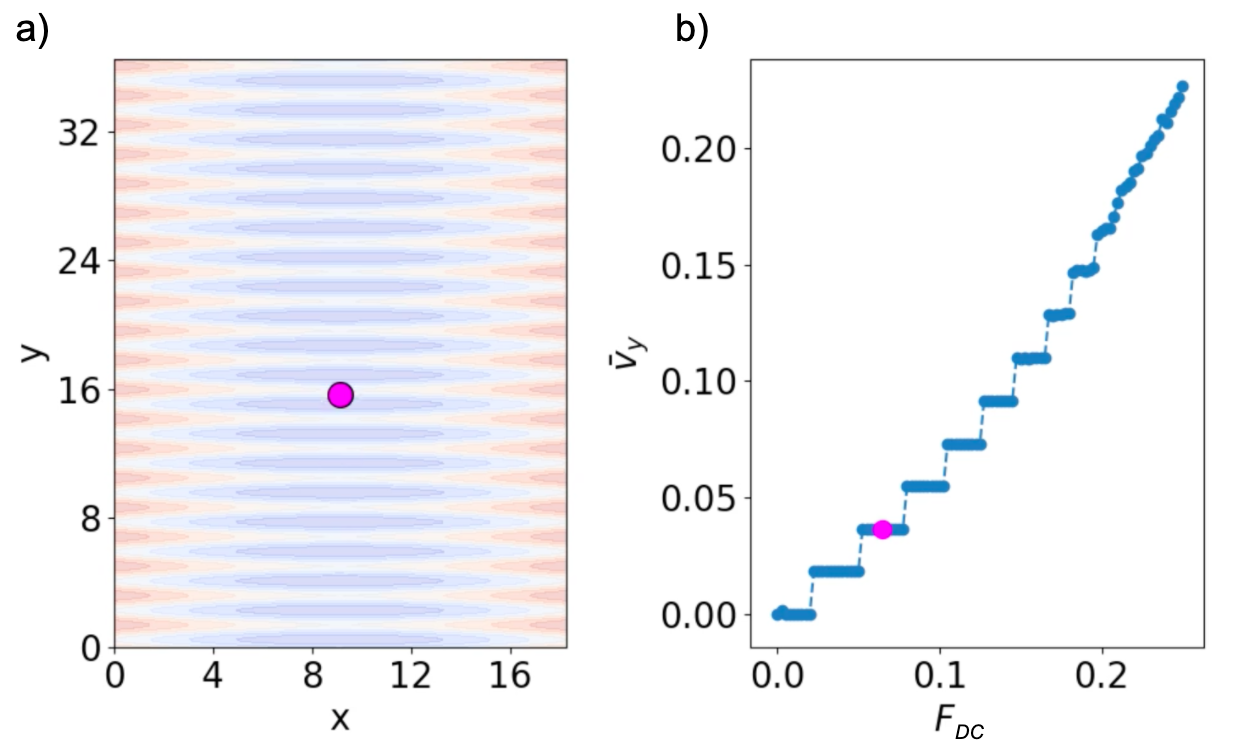
\includegraphics[scale=.25]{single}
\caption{\textbf{(a)} The particle is driven with a constant $F_{AC}$ and $f$ through a periodic potential landscape where blue are minima and red are maxima in the potential. \textbf{(b)} An average particle velocity in the y-direction $\bar{v}_{y}$ as a function of the driving force $F_{DC}$. In the animation the magenta dot represents the $\bar{v}_{y}$ at which the particle in Fig. 1a) is moving.}
\end{figure}
\end{center}

\subsection{Synchronization in multi-particle systems}
\label{sec:sync}

We simulated a twenty particle system confined to a narrow channel, as shown in Fig. 2a). The interparticle forces of neighboring particles cause the system to form a buckled chain when the system is annealed. When a single particle is driven, the neighboring particles act similarly to a periodic landscape to impede its motion. A driven particle can exhibit mode locking with a well-chosen AC drive and frequency. In the attached movie, Figure2.mp4, we show the complex dynamics of mode locking, where the driven particle leap-frogs past the other particles. 

\begin{center}
\begin{figure}[h!]
\centering
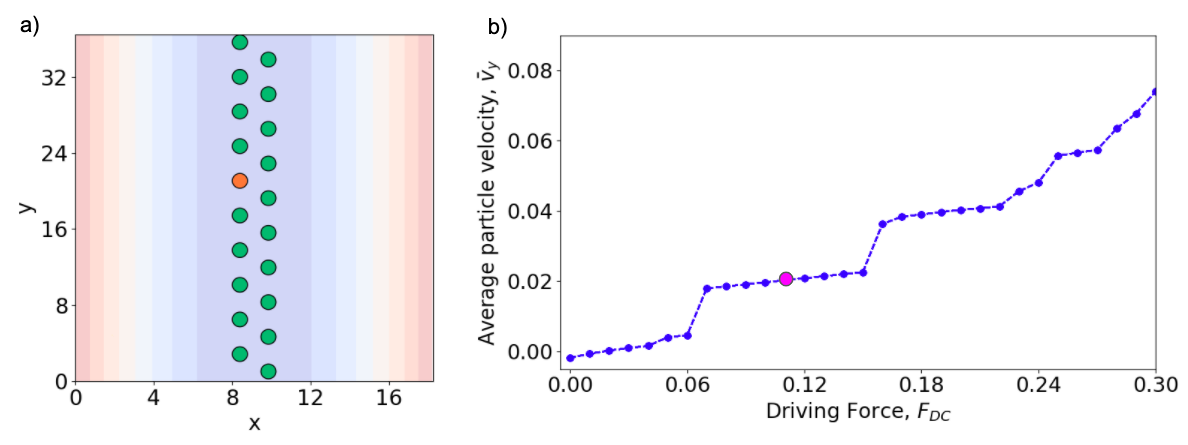
\includegraphics[scale=.40]{twenty}
\caption{\textbf{(a)} The orange particle is driven with a constant $F_{AC}$ and $f$ through 19 particles, colored green, confined by a quasi one-dimensional channel. The landscape is colored as in Fig. 1. \textbf{(b)} $\bar{v}_{y}$ versus $F_{DC}$, where $\bar{v}_{y}$ is the average particle velocity of the driven particle in the y-direction.}
\end{figure}
\end{center}

\subsection{Kinked system}
\label{sec:static}	% You can label sections for reference




\section{Quasiperiodic substrate}
\label{sec:quasiperiod}	% You can label sections for reference

\section{Chaotic dynamics}
\label{sec:chaos}	% You can label sections for reference

\section{Associated problems}



\section{Conclusion}




\begin{acknowledgments}

We acknowledge Harvey Gould and Jan Tobochnik, who supported our development of this article.  We acknowledge funding from the M.J. Murdock Charitable Trust and the Pacific PRISM program.

\end{acknowledgments}


\begin{thebibliography}{99}
% The numeral (here 99) in curly braces is nominally the number of entries in
% the bibliography. It's supposed to affect the amount of space around the
% numerical labels, so only the number of digits should matter--and even that
% seems to make no discernible difference.

\bibitem{juniper2015} M. P. N. Juniper, A. V. Straube, R. Besseling, D. G. A. L. Aarts, and R. P. A. Dullens, Microscopic dynamics of synchronization in driven colloids. Nat. Commun. 6, 7187 (2015).

%\bibitem{latexsite} \LaTeX\ Project Web Site, \url{<http://www.latex-project.org/>}.

%\bibitem{wikibook} \textit{\LaTeX} (Wikibook), \url{<http://en.wikibooks.org/wiki/LaTeX/>}.

%\bibitem{latexbook}Helmut Kopka and Patrick W. Daly, \textit{A Guide to
%\LaTeX}, 4th edition (Addison-Wesley, Boston, 2004).

%\bibitem{revtex} REV\TeX\ 4 Home Page, \url{<https://authors.aps.org/revtex4/>}.

%\bibitem{cloudLaTeX} On the other hand, you can avoid the installation process
%entirely by using a cloud-based \LaTeX\ processor such as ShareLaTeX,
%\url{<https://www.sharelatex.com/>}, or write\LaTeX, \url{<https://www.writelatex.com/>}.

%\bibitem{nevermindlogic} In typography, aesthetics often takes precedence over logic.

%\bibitem{FontEncodingComment} Please don't try to handle foreign characters 
%and accents with the \texttt{inputenc} and \texttt{fontenc} packages, which 
%are incompatible with AJP's editing process.

%\bibitem{wikimathpage} See the Mathematics chapter of Ref.~\onlinecite{wikibook} for an excellent overview of math symbols and equations, with examples.

%\bibitem{labelnames} Thinking up a good label name takes a moment, but 
%it's worth the trouble; we strongly advise against using labels like 
%\texttt{eq2}, which become extremely confusing after you decide to add 
%another equation before Eq.~(\ref{deriv}).

%\bibitem{footnotes} You need to process a file twice to get the counters correct.

%\bibitem{mermin} N. David Mermin, ``What's wrong with these equations?,'' 
%Phys. Today \textbf{42} (10), 9--11 (1989).  
% Note that the issue number (10) in this citation is required, because
% each issue of Physics Today starts over with page 1.  Also note the use of
% an en-dash (--), not a hyphen (-), for the page range.

%\bibitem{editorsite} American Journal of Physics Editor's Web Site, 
%\url{<http://ajp.dickinson.edu>}.

%\bibitem{feynman} Richard P. Feynman, Robert B. Leighton, and Matthew Sands, 
%\textit{The Feynman Lectures on Physics, Vol.\ 1} (Addison-Wesley, 1964), p.~3-10.
% Note that this book is paginated by chapter; "3-10" is a single page reference
% that uses a hyphen, not a range of pages that would us an en-dash (--).

%\bibitem{noBIBTeX} Many \LaTeX\ users manage their bibliographic data with 
%a tool called BIB\TeX.  Unfortunately, AJP cannot accept BIB\TeX\ files; all 
%bibliographic references must be incorporated into the manuscript file
%as shown here, at least when you send an editable file for production.

%\bibitem{dyson} Freeman J. Dyson, ``Feynman's proof of the Maxwell equations,''
%Am. J. Phys. \textbf{58} (3), 209--211.  
% The issue number (3) in this citation is optional, because AJP's pagination 
% is by volume.

%\bibitem{examplevolume} M. R. Flannery, ``Elastic scattering,'' in 
%\textit{Atomic, Molecular, and Optical Physics Handbook}, edited by
%G. W. F. Drake (AIP Press, New York, 1996), p.~520.

%\bibitem{AIPstylemanual} \textit{AIP Style Manual}, 4th edition (American 
%Institute of Physics, New York, 1990). Available online at 
%\url{<http://www.aip.org/pubservs/style/4thed/toc.html>}. Although parts of 
%it have been made out of date by advancing technology, most of this manual 
%is still as useful as ever. Just be sure to follow AJP's specific rules
%whenever they conflict with those in the manual.

\end{thebibliography}

% If your manuscript is conditionally accepted, the editors will ask you to
% submit your editable LaTeX source file.  Before doing so, you should move
% all tables and figure captions to the end, as shown below.  Tables come 
% first, followed by figure captions (with figure inclusions commented-out).
% Figures should be submitted as separate files, collected with the
% LaTeX file into a single .zip archive.

%\newpage   % Start a new page for tables

%\begin{table}[h!]
%\centering
%\caption{Elementary bosons}
%\begin{ruledtabular}
%\begin{tabular}{l c c c c p{5cm}}
%Name & Symbol & Mass (GeV/$c^2$) & Spin & Discovered & Interacts with \\
%\hline
%Photon & $\gamma$ & \ \ 0 & 1 & 1905 & Electrically charged particles \\
%Gluons & $g$ & \ \ 0 & 1 & 1978 & Strongly interacting particles (quarks and gluons) \\
%Weak charged bosons & $W^\pm$ & \ 82 & 1 & 1983 & Quarks, leptons, $W^\pm$, $Z^0$, $\gamma$ \\
%Weak neutral boson & $Z^0$ & \ 91 & 1 & 1983 & Quarks, leptons, $W^\pm$, $Z^0$ \\
%Higgs boson & $H$ & 126 & 0 & 2012 & Massive particles (according to theory) \\
%\end{tabular}
%\end{ruledtabular}
%\label{bosons}
%\end{table}

%\newpage   % Start a new page for figure captions

%\section*{Figure captions}

%\begin{figure}[h!]
%\centering
%\includegraphics{GasBulbData.eps}   % This line stays commented-out
%\caption{Pressure as a function of temperature for a fixed volume of air.  
%The three data sets are for three different amounts of air in the container. 
%For an ideal gas, the pressure would go to zero at $-273^\circ$C.  (Notice
%that this is a vector graphic, so it can be viewed at any scale without
%seeing pixels.)}

%\label{gasbulbdata}
%\end{figure}

%\begin{figure}[h!]
%\centering
%\includegraphics[width=5in]{ThreeSunsets.jpg}   % This line stays commented-out
%\caption{Three overlaid sequences of photos of the setting sun, taken
%near the December solstice (left), September equinox (center), and
%June solstice (right), all from the same location at 41$^\circ$ north
%latitude. The time interval between images in each sequence is approximately
%four minutes.}
%\label{sunsets}
%\end{figure}

\end{document}
